\section{Implementación}

\subsection{Montaje Físico y Componentes}
El circuito se ensambló en un protoboard, utilizando la placa de desarrollo **Arduino Uno** como unidad de control central. La arquitectura de diseño se centró en la gestión eficiente de los periféricos, que incluyeron:

\begin{itemize}
        \item \textbf{Matriz LED $8\times8$}: Controlada indirectamente a través de registros de desplazamiento serial-paralelo (74LS595 para filas y un registro complementario para columnas), lo que permitió minimizar el uso de pines digitales del microcontrolador.
            \item \textbf{Joystick}: Las salidas analógicas se conectaron a los pines \texttt{A0} y \texttt{A1} del Arduino. El botón se conectó al pin \texttt{D2} para la captura de eventos de inicio de juego mediante una interrupción \textit{hardware}.
                \item \textbf{Display LCD1602 (I2C)}: Se utilizó la interfaz I2C para la comunicación con el display (líneas SDA y SCL), simplificando el cableado y la gestión de la interfaz de usuario.
\end{itemize}

El montaje requirió la conexión en cascada de los registros de desplazamiento para la matriz, verificando la secuencia de \texttt{shiftOut} para asegurar que cada bit se mapeara a su respectivo LED en la matriz física.

\begin{figure}[h]
        \centering
            \caption{Montaje físico del circuito de juego (Joystick, LCD y Matriz LED).}
                \label{fig:montaje_fisico}
                    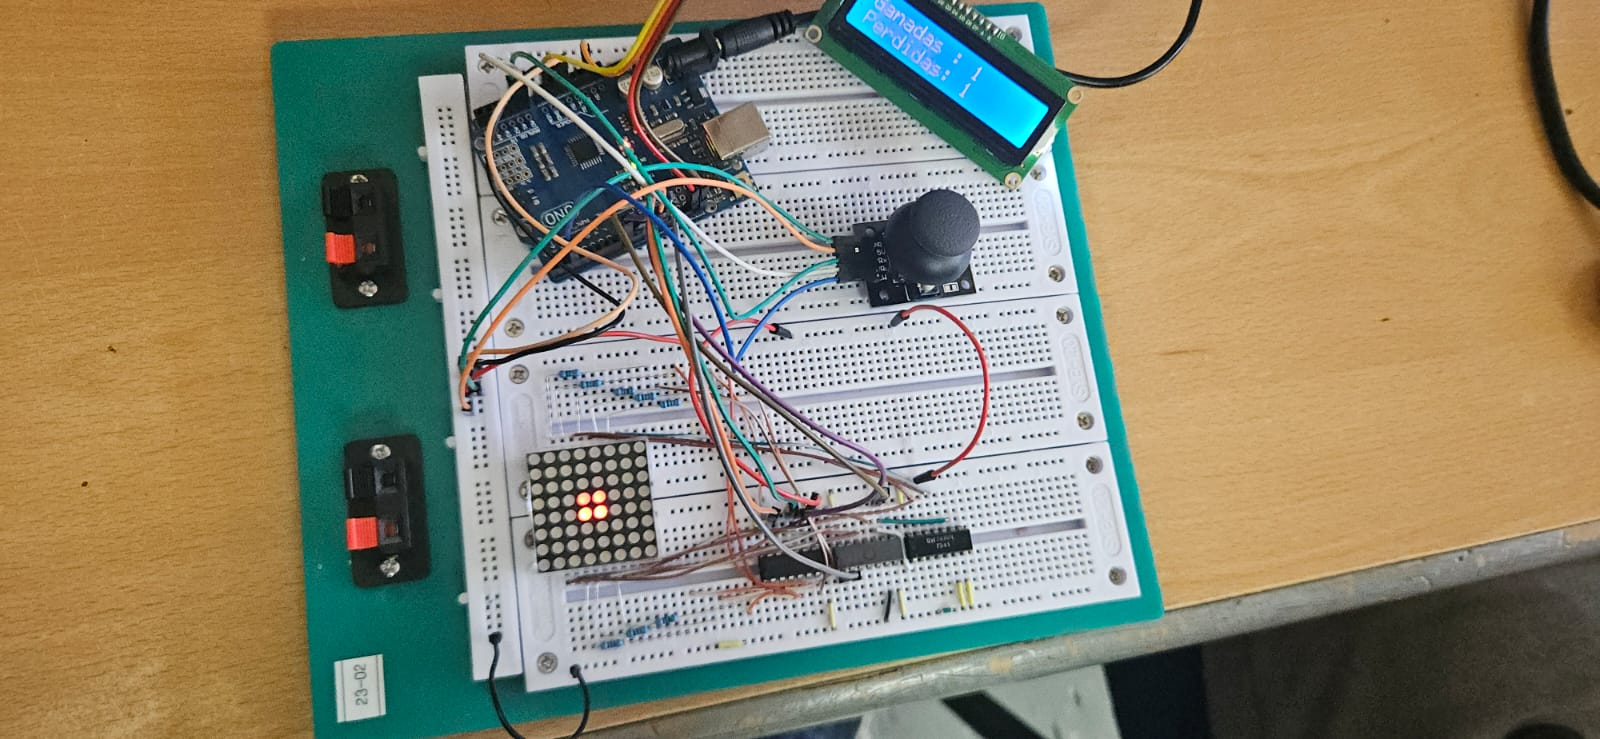
\includegraphics[width=0.8\linewidth]{Diagramas/Imagen de WhatsApp 2025-09-26 a las 22.01.48_a38513c5.jpg}
\end{figure}

